\documentclass[UTF8,zihao=-4]{ctexart}
\usepackage[a4paper,margin=2.5cm]{geometry}
\usepackage{amsmath, amssymb, amsthm}
\usepackage{bm}
\usepackage{hyperref}
\usepackage{graphicx}
\usepackage{caption}
\usepackage{listings}
\usepackage{xcolor}
\usepackage{float}
\usepackage{booktabs}
\usepackage{longtable}
\usepackage{multirow}
\usepackage{placeins}
\graphicspath{{figures/}}

% 代码样式
\lstdefinestyle{code}{
  basicstyle=\ttfamily\small,
  numbers=left,
  numberstyle=\tiny,
  numbersep=8pt,
  keywordstyle=\color{blue},
  commentstyle=\color{teal!70!black},
  stringstyle=\color{orange!70!black},
  showstringspaces=false,
  breaklines=true,
  frame=single,
  framerule=0.3pt,
  rulecolor=\color{black!15}
}
\lstset{style=code}

\title{评测与可解释性:基准体系、评测维度与注意力归因分析}
\author{}
\date{\today}

\begin{document}
\maketitle

\section{Benchmark:MMLU, GSM8K, BIG-Bench}
\subsection{主流基准概览}
图\ref{fig:benchmark_landscape_cn} 将 MMLU、GSM8K、BIG-Bench 放在同一谱系中:从知识覆盖到复杂推理,再到长尾能力与安全探测,形成多维度评测组合。
\begin{figure}[H]
  \centering
  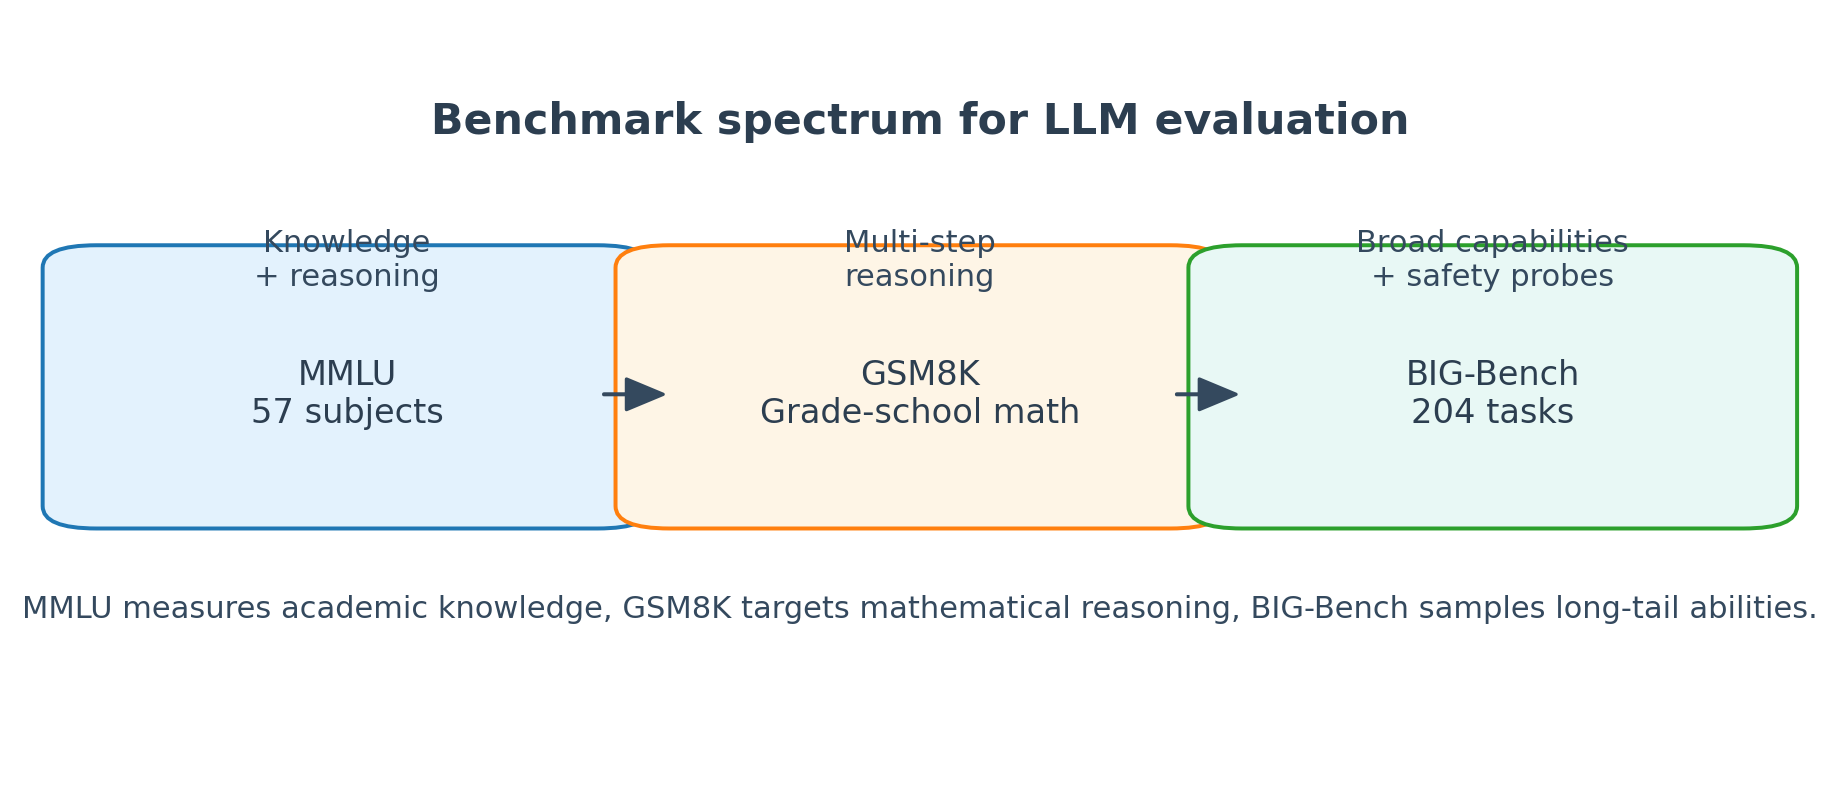
\includegraphics[width=0.9\textwidth]{benchmark_landscape.png}
  \caption{基准谱系:MMLU(广域知识)、GSM8K(多步推理)、BIG-Bench(长尾任务与安全评估)。}
  \label{fig:benchmark_landscape_cn}
\end{figure}

\subsection{MMLU(Massive Multitask Language Understanding)}
\begin{itemize}
  \item 覆盖 57 个学科领域(STEM、Humanities、Social Sciences 等),共 15K 问题;
  \item 采用四选一形式,评估模型的知识记忆与跨学科能力;
  \item 常见扩展:翻译测试、few-shot 引导、chain-of-thought 解析。
\end{itemize}

\subsection{GSM8K}
\begin{itemize}
  \item 8K 小学数学题,强调逐步逻辑推导;
  \item 通常结合 CoT prompting、多样性采样(self-consistency)提升准确率;
  \item 可扩展到 GSM-Hard、math word problems、program-aided solutions。
\end{itemize}

\subsection{BIG-Bench / BIG-Bench Hard}
\begin{itemize}
  \item 204 个任务,涵盖语言、常识、伦理、定制逻辑;
  \item 引入 crowdsourced 任务与 adversarial 题目,测试泛化与鲁棒性;
  \item BIG-Bench Hard 聚焦人类可轻松解决但模型困难的题型,是模型突破的前沿指标。
\end{itemize}

\section{评测维度:知识、推理、安全、价值观}
\subsection{维度拆解}
\begin{longtable}{p{3cm}p{4cm}p{6cm}}
\toprule
维度 & 代表基准 & 评测重点 \\
\midrule
知识(Knowledge) & MMLU, TruthfulQA & 事实记忆、专业知识、时效性 \\
推理(Reasoning) & GSM8K, ARC-Challenge, MathBench & 多步推导、符号运算、规划与策略 \\
安全(Safety) & RealToxicity, AdvBench, JailbreakBench & 有害内容、越狱、滥用场景识别 \\
价值观(Values Alignment) & Anthropic Helpful-Harmless, Constitutional AI eval & 道德取向、文化敏感性、价值一致性 \\
\bottomline
\end{longtable}

\subsection{评测流程建议}
\begin{enumerate}
  \item 建立离线评测集(静态基准 + 自定义场景),定期运行;
  \item 结合在线日志(用户反馈、拒绝率)形成闭环;
  \item 引入自动化报告:指标趋势、异常检测、SLA 监控;
  \item 对安全与价值观评测采用红队(red teaming)策略,持续更新题库。
\end{enumerate}

\subsection{指标与可视化}
\begin{itemize}
  \item 精度类:Accuracy、macro/micro F1、Exact Match;
  \item 推理链分析:思路长度、错误类型、工具调用次数;
  \item 安全类:拒绝率、违规触发率、恢复率(是否能自我纠正);
  \item 价值观类:正负面反馈比例、跨文化一致性。
\end{itemize}

\section{注意力可视化与 Attribution 分析}
\subsection{解释性流程}
图\ref{fig:interpretability_pipeline_cn} 描述了从输入、注意力探测、归因计算到可视化洞察的完整管线。
\begin{figure}[H]
  \centering
  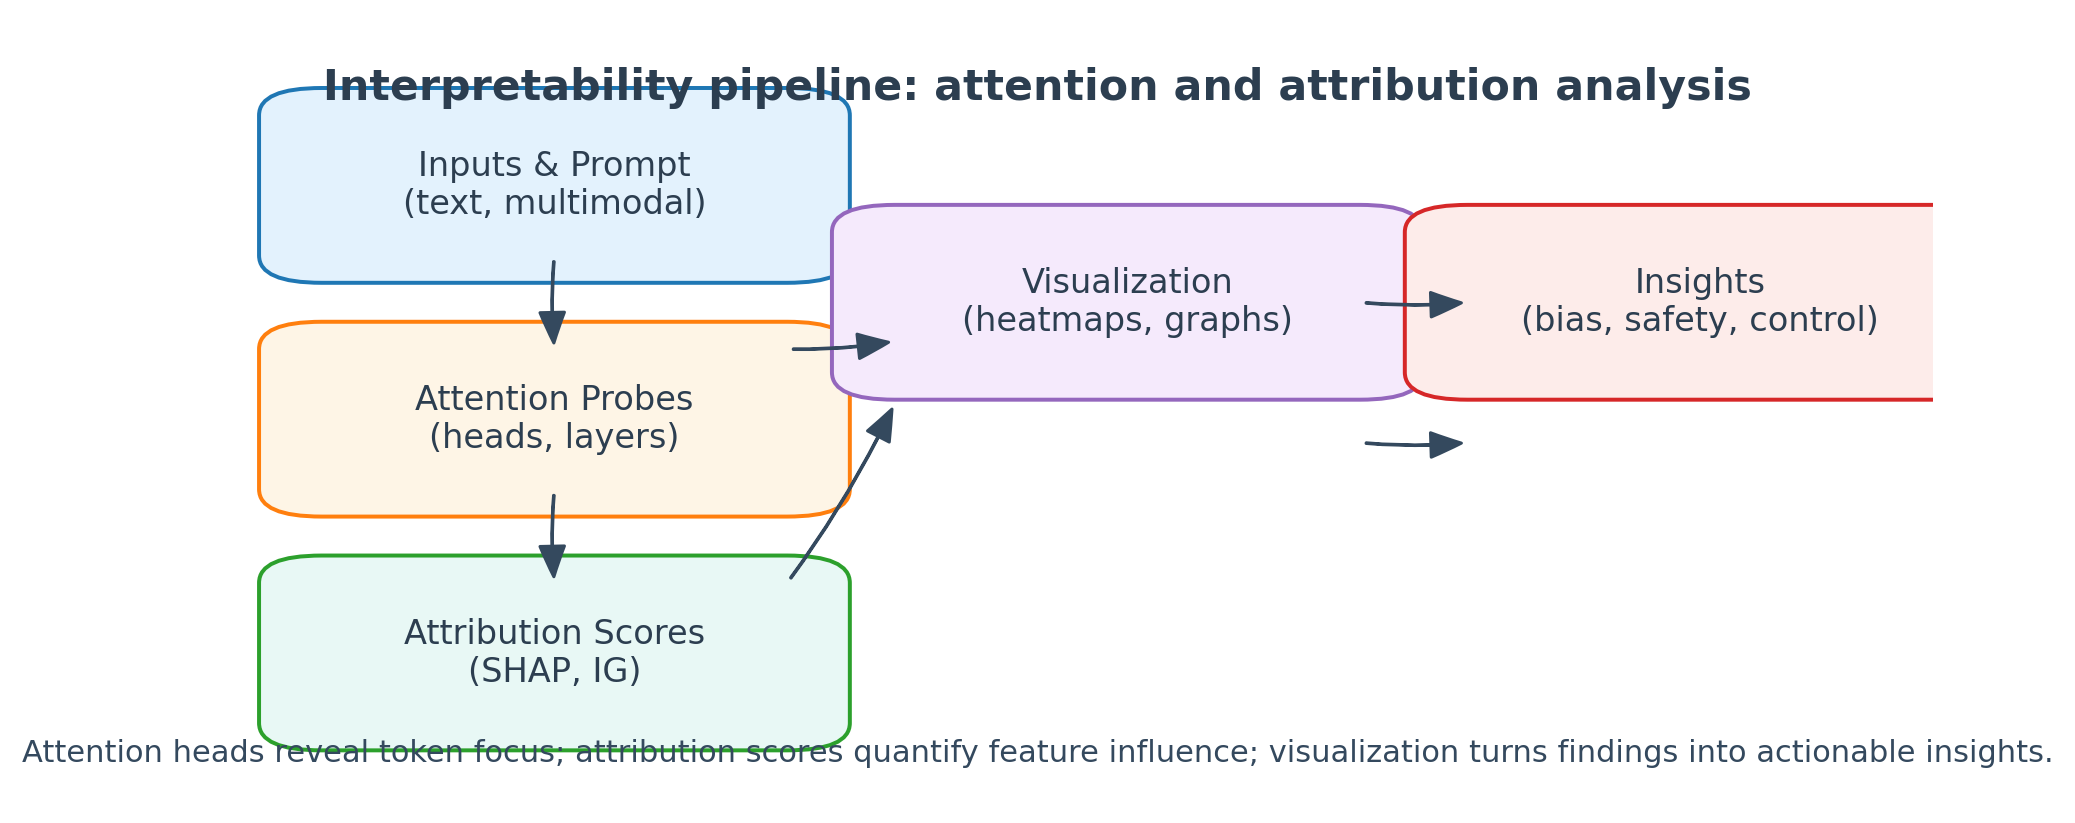
\includegraphics[width=0.9\textwidth]{interpretability_pipeline.png}
  \caption{可解释性流程:输入 \textrightarrow{} 注意力探测 \textrightarrow{} 归因得分 \textrightarrow{} 可视化 \textrightarrow{} 洞察。}
  \label{fig:interpretability_pipeline_cn}
\end{figure}

\subsection{注意力分析}
\begin{itemize}
  \item \textbf{Attention Rollout:} 将多层注意力矩阵相乘计算整体依赖;
  \item \textbf{Attention Flow:} 结合残差与前馈层,更准确反映信息流动(Chefer 等);
  \item \textbf{Head Importance:} 通过梯度、L0 正则评估注意力头的重要性,可指导剪枝。
\end{itemize}

\subsection{归因方法}
\begin{itemize}
  \item \textbf{Integrated Gradients (IG):} 沿输入路径积分梯度,衡量特征贡献;
  \item \textbf{SHAP:} 基于博弈论的特征贡献分配,支持多模态与 tabular;
  \item \textbf{Layer-wise Relevance Propagation (LRP):} 在深层网络中逐层传播相关度。
\end{itemize}

\subsection{实践示例:Integrated Gradients}
\begin{lstlisting}[language=Python,caption={对 LLaMA 进行 Integrated Gradients 归因分析}]
import torch
from transformers import AutoModelForCausalLM, AutoTokenizer
from captum.attr import IntegratedGradients

model_name = "meta-llama/Llama-2-7b-chat-hf"
tokenizer = AutoTokenizer.from_pretrained(model_name)
model = AutoModelForCausalLM.from_pretrained(model_name, torch_dtype=torch.float16).cuda()
model.eval()

prompt = "Explain why the sky is blue."
inputs = tokenizer(prompt, return_tensors="pt").to(model.device)

def forward_func(input_ids, attention_mask):
    outputs = model(input_ids=input_ids, attention_mask=attention_mask)
    # 取最后一个 logit 代表回答品质
    return outputs.logits[:, -1, :].max(dim=-1).values

ig = IntegratedGradients(forward_func)
baseline = torch.zeros_like(inputs["input_ids"])
attributions, _ = ig.attribute(
    inputs["input_ids"],
    baselines=baseline,
    additional_forward_args=(inputs["attention_mask"],),
    return_convergence_delta=True,
)

tokens = tokenizer.convert_ids_to_tokens(inputs["input_ids"][0])
for token, score in zip(tokens, attributions[0].sum(dim=-1).tolist()):
    print(f"{token}: {score:.4f}")
\end{lstlisting}

\subsection{可视化与用户界面}
\begin{itemize}
  \item \textbf{热力图:} 将 token 重要度叠加在文本上,直观展示关注焦点;
  \item \textbf{图结构:} 使用 networkx/graphviz 展示注意力流向;
  \item \textbf{交互式仪表盘:} Streamlit/Gradio 构建交互界面,允许筛选样本、比较模型。
\end{itemize}

\section*{实践建议}
\begin{itemize}
  \item 将评测维度与业务目标对齐:知识 + 推理 + 安全 + 价值观形成闭环;
  \item 构建评测基准仓库,统一数据格式、prompt 模板与报告输出;
  \item 结合解释性工具分析模型失败案例,识别幻觉、偏见、推理链断裂;
  \item 在发布前进行红队与灰盒测试,并记录模型行为以备审计。
\end{itemize}

\section*{参考文献}
\begin{itemize}
  \item Hendrycks et al. ``Measuring Massive Multitask Language Understanding.'' ICLR, 2021.
  \item Cobbe et al. ``Training Verifiers to Solve Math Word Problems.'' arXiv, 2021.
  \item Srivastava et al. ``Beyond the Imitation Game Benchmark (BIG-bench).'' arXiv, 2022.
  \item Chefer et al. ``Transformers Interpretability Beyond Attention Visualization.'' CVPR, 2021.
  \item Mukherjee et al. ``LLM Introspection: Improving Safety via Interpretability.'' arXiv, 2023.
\end{itemize}

\end{document}

